\section{Auswertung}
\label{sec:Auswertung}

\subsection{Vorbereitung}

Die Größen Ordnungszahl $Z$, Literaturwert der
K-Kante $E_\text{K}^\text{Lit}$, der zugehörige Glanzwinkel 
$\theta_\text{glanz}^\text{Lit}$ und die Abschirmkonstante 
$\sigma_\text{K}$ verschiedener Elemente sind in Tabelle 
\ref{tab:literatur} aufgelistet.

\begin{table}
  \centering
  \caption{Literaturwerte und daraus errechnete Größen verschiedener Elemente}
  \label{tab:literatur}
  \sisetup{table-format=2.1}
  \begin{tabular}{c c c c c}
  \toprule
  $ $ & $Z$ & $E_\text{K}^\text{Lit} \,/\, \si{\kilo\eV}$
  & $\theta_\text{glanz}^\text{Lit} \,/\, \si{\degree}$ & 
  $\sigma_\text{k}$\\
  \midrule 
  Cu & 29 & 08,98 & 20,05 & 3,30 \\
  Zn & 30 & 09,65 & 18,60 & 3,36 \\
  Ge & 32 & 11,10 & 16,10 & 3,43 \\
  Br & 35 & 13,47 & 13,22 & 3,53 \\
  Rb & 37 & 15,19 & 11,69 & 3,58 \\
  Sr & 38 & 16,10 & 11,03 & 3,60 \\
  Zr & 40 & 18,00 & 09,85 & 3,62 \\
  Nb & 41 & 18,99 & 09,33 & 3,63 \\
  Au & 79 & 80,77 & 02,18 & 1,94 \\
  \bottomrule
  \end{tabular}
  \end{table}

Dabei ergibt sich der Glanzwinkel

  \begin{equation}
    \theta_\text{glanz} = \text{arcsin}\left(\frac{h \cdot c}{E \cdot 2d}\right)
    \label{eqn:theta}
  \end{equation}

  durch die Umstellung der Gleichung \eqref{eqn:Bragg} und durch Einsetzen 
  des Ausdrucks $\lambda = \frac{h \cdot c}{E}$. Weiterhin beträgt die Gitterkonstante
  des Kristalls $d_\text{LiF} = \SI{201.4}{\pico\meter}$.

  Die Abschirmkonstante $\sigma_\text{K}$ ergibt sich für die K-Schale aus Gleichung
  \eqref{eqn:std} durch Einsetzen des Ausdrucks $z_\text{eff} = z -\sigma$ und durch 
  Umstellung zu 

  \begin{equation}
    \sigma_\text{K} = z - \sqrt{\frac{E_n}{R_{\infty}}} \; .
  \end{equation}

  Weiterhin sind zur Überprüfung der Absorption die folgeneden Werte für Kupfer 
  ermittelt worden:

  \begin{align*}
    \text{Für } K_\alpha \text{ : } E_{K_\alpha} &= \SI{8.046}{\kilo\eV}, \\
    \text{Für } K_\beta \text{ : } E_{K_\beta} &= \SI{8.904}{\kilo\eV} \\
    \theta_{K_\alpha} &= \SI{22.49}{\degree}, \\
    \theta_{K_\beta} &= \SI{20.22}{\degree} \: .
 \end{align*}




  %https://wissen.science-and-fun.de/tabellen-fur-spektroskopiker/wellenlaengen-und-anregungsenergien-von-k-und-l-absorptionskanten/





\subsection{Überprüfung der Bragg Bedingung}

Nach der Braggbedingung ist zu erwarten, dass das gemessene Intensitätsmaximum
für einen bestimmten Glanzwinkel auftritt. 
Dies wird durch Abbildung ... verifiziert. In jener ist eindeutig ein Maximum 
mit etwa $310$ Impulsen bei $\SI{27.25}{\degree}$ zu erkennen.

\subsection{Das Emissionsspektrum einer Kupferröntgenröhre}

\subsection{Das Emissionsspektrum einer Kupferröntgenröhre}

Das gemessene Emissionsspektrum der Kupferanode ist in Abbildung ... abgebildet.
In dieser sind mit zunehmendem Winkel gut der Grenzwinkel bei etwa $\SI{5}{\degree}$,
der Bremsberg im bereich von $\SI{5}{\degree}$ bis $\SI{19}{\degree}$, die 
$K_\alpha$-Kante bei etwa $\SI{20}{\degree}$ und die $K_\beta$-Kante bei 
etwa $\SI{22.5}{\degree}$ zu erkennen.









%\begin{figure}
%  \centering
%  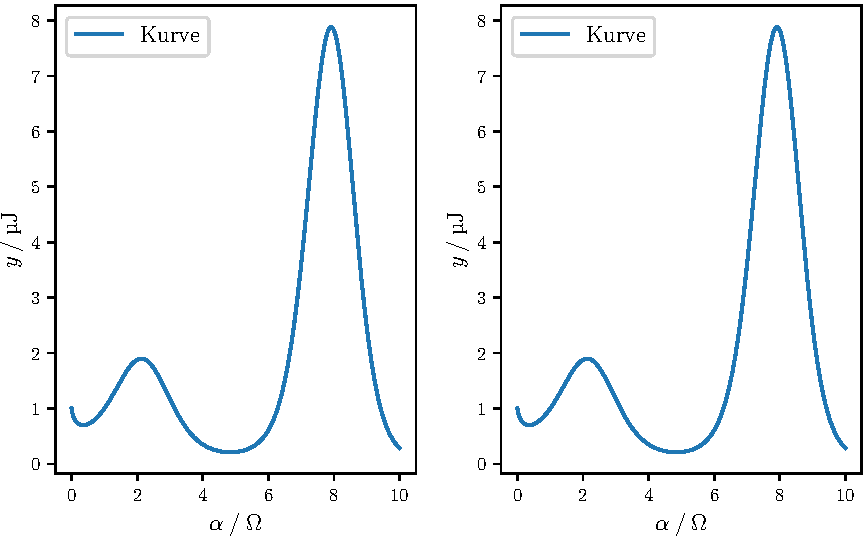
\includegraphics{plot.pdf}
%  \caption{Plot.}
%  \label{fig:plot}
%\end{figure}
